\documentclass[11pt]{article}
\usepackage[margin=1in]{geometry}
\usepackage[T1]{fontenc}
\usepackage{lmodern}
\usepackage{amsmath,amssymb,booktabs,array,graphicx,float}
\usepackage{hyperref}
\setlength{\emergencystretch}{8em}
\renewcommand{\arraystretch}{1.3}
\makeatletter
\newcommand{\sha}{\begingroup\catcode`\_=12 \sha@read}
\newcommand{\sha@read}[1]{\ttfamily\sha@loop#1\relax\endgroup}
\def\sha@loop#1{%
  \ifx\relax#1\else
    #1\allowbreak
    \expandafter\sha@loop
  \fi}
\makeatother
\hypersetup{colorlinks=true,linkcolor=blue,urlcolor=blue,citecolor=blue,
  pdftitle={Replication of the polytomous person-fit Monte Carlo in Beck (2023)},
  pdfauthor={}}
\newcommand{\proofbase}{https://github.com/alectionary/vibe-math/blob/master/formalization/polytomous-person-fit}
\makeatletter
\def\pf@show#1{%
  \ifx\relax#1\else
    #1\allowbreak
    \expandafter\pf@show
  \fi}
\newcommand{\src}{\begingroup\catcode`\_=12 \pf@src}
\newcommand{\pf@src}[1]{%
  \edef\srcurl{\proofbase/#1}%
  \href{\srcurl}{\texttt{\pf@show#1\relax}}\endgroup}
\newcommand{\srcat}{\begingroup\catcode`\_=12 \pf@srcat}
\newcommand{\pf@srcat}[2]{%
  \edef\srcurl{\proofbase/#1\#L#2}%
  \href{\srcurl}{\texttt{\pf@show#1\relax}}\endgroup}
\newcommand{\srcdir}{\begingroup\catcode`\_=12 \pf@dir}
\newcommand{\pf@dir}[1]{%
  \edef\srcurl{https://github.com/alectionary/vibe-math/tree/master/formalization/polytomous-person-fit/#1}%
  \href{\srcurl}{\texttt{\pf@show#1\relax}}\endgroup}
\makeatother

\title{Replication of the polytomous person-fit Monte Carlo\\
in Beck (2023)}
\author{}
\date{29 October 2026}

\begin{document}
\maketitle

\begin{abstract}
Do the detection rates in Beck (2023) follow from the Monte Carlo
described there?
The dissertation's headline result is the sensitivity of \(U3\), the
normed number of Guttman errors, and \(H_i^T\) for each of six bias
types.
This note recomputes the printed ANOVA tables and reruns the
classification rates from that design, supplying the inputs the
dissertation does not print.
None of the eighteen grand sensitivities fall inside a
two-standard-error band, before or after Holm.
Careless responding comes out between \(0.44\) and \(0.50\), against
the printed \(0.29\).
The nearest misses, at an extreme-response constant \(\varepsilon=0.5\),
are the normed Guttman errors for midpoint responding, \(0.0035\)
against a printed \(0.00\), and for extreme responding, \(0.284\)
against \(0.27\).
The likely causes are unpublished inputs: the \texttt{ltm} thresholds
and the missing seven-option boundary row, the boundary draw and its
seed, the magnitude of \(\varepsilon\), and the fraction of items
replaced when responding is careless.
A second generator, the package versions current in May~2023, the
Monte Carlo standard errors, and the person-fit formulas do not
account for those misses.
The ANOVA effect sizes do replicate.
All \(504\) partial omega squared values agree with the printed \(F\)
statistics at \(N=32{,}000\), to within \(0.005\).
Specificity, negative predictive value, and positive predictive value
largely follow from flagging \(5\%\) of respondents.
Specificity and negative predictive value sit within \(0.006\) of that
identity, and positive predictive value sits within \(0.02\).
\end{abstract}

\section{The question, and the headline}
\label{sec:headline}

This section answers whether the printed detection rates come from the
Monte Carlo in the dissertation.
Beck's headline result is the sensitivity of \(U3\), the normed number
of Guttman errors, and \(H_i^T\) for each of six bias types.
The rerun uses the printed design and supplies the inputs the
dissertation does not print.
Beck's headline sensitivities did not replicate, under the assumptions
stated below.
None of the eighteen grand sensitivities fall inside a
two-standard-error band, before or after Holm.
Careless responding comes out between \(0.44\) and \(0.50\), against
the printed \(0.29\).
The nearest misses are the normed Guttman errors for midpoint
responding, \(0.0035\) against \(0.00\), and for extreme responding,
\(0.284\) against \(0.27\), at \(\varepsilon=0.5\).
The likely causes are unpublished inputs: the \texttt{ltm} thresholds
and the seven-option row, the boundary draw and its seed, the
extreme-response constant \(\varepsilon\), and the careless-item
fraction.
The generator, the package versions, Monte Carlo noise, and the
person-fit implementations were checked and do not account for the
misses.
The ANOVA effect sizes do replicate.
Specificity, negative predictive value, and positive predictive value
largely follow from flagging \(5\%\) of respondents, and those printed
rates sit close to that identity.

Beck (2023) \cite{beck2023} studies whether three nonparametric
person-fit statistics detect response bias on ordered polytomous items.
The design is six bias types, four numbers of response options, four
dimensionalities, and two test lengths: \(192\) conditions.
Each condition has \(900\) ordinary respondents and \(100\) biased
respondents, repeated \(1{,}000\) times.
The statistics are \(U3\), the normed number of Guttman errors, and the
person coefficient \(H_i^T\).
The cutoff in each replication is the median of the 5th percentiles of
\(1{,}000\) bootstrap samples.
Tables~A24--A26 collect the rates.
Sensitivities run from \(0.00\), for midpoint responding on the normed
Guttman errors and on \(U3\), to \(0.29\), for careless responding on
the normed Guttman errors.
Specificities run from \(0.94\) to \(0.98\).

The generative rerun does not land on the sensitivity column.
The reported run uses the linear predictor in Equation~23 as printed,
\(40\) replications, and an extreme-response constant \(\varepsilon=0.5\).
Of the eighteen grand sensitivities, none fall inside a two-standard-error
band, before or after Holm.
The normed Guttman errors come nearest: midpoint responding is
\(0.0035\) against \(0.00\), and extreme responding is \(0.284\) against
\(0.27\).
The combined standard errors are \(0.00018\) and \(0.00088\).
Two factor-margin cells do match, and two more sit just outside the
band.
\(U3\), computed from the same definition as PerFit~1.4.7, does not
follow the printed \(U3\) column on either tail.
Beck (2015) \cite{beck2015}, cited for the moments, was not available
on the first attempt to fetch it.
The copy obtained after that failure prints scale correlations and
factor loadings, not graded thresholds.
Using those correlations in place of Table~A1 moves the normed-Guttman
rates by less than \(0.01\).
A hand-written graded sampler, run for the same \(40\) replications,
puts none of the eighteen grand sensitivities inside the band.
The largest gap between that sampler and \texttt{mirt} on a grand
sensitivity is \(0.0041\).
PerFit~1.4.6, the release current in May~2023, and mokken~3.0.6 score
the same matrices as PerFit~1.4.7 and mokken~3.1.2.

Two checks use only the printed numbers.
Partial omega squared, computed from each printed \(F\) at
\(N=32{,}000\), matches all \(504\) entries in Tables~C1--C18 to within
\(0.005\), which is the half-unit of the printed two-decimal column.
When exactly \(50\) of \(1{,}000\) people are flagged and \(100\) of them
are the biased respondents, specificity, positive predictive value, and
negative predictive value are functions of sensitivity.
Those three rates largely follow from flagging \(5\%\) of respondents.
Specificity and negative predictive value in Tables~A24--A26 sit within
\(0.006\) of that identity.
Positive predictive value sits within \(0.02\).

The original work is the design, the bias definitions, and the printed
tables.
The calculations below are ours: the arithmetic checks, the Monte Carlo,
and the comparison.
Multiplicity is applied only to our check that a printed rate and our
rate agree.
The dissertation's own tests are one classification per replication.

\section{What we replicated}
\label{sec:replicated}

This section answers which printed claims agree with a direct
calculation.
Beck's headline sensitivities do not.
None of the eighteen grand sensitivities fall inside a
two-standard-error band, before or after Holm.
The ANOVA effect sizes do.
Specificity, negative predictive value, and positive predictive value
largely follow from flagging \(5\%\) of respondents, and those printed
rates sit close to that identity.
Table~\ref{tab:compare} is that comparison.
``Match'' means the same number, or a Monte Carlo gap no larger than
two combined standard errors.
``Partial'' means one piece of the claim holds and another does not.
``Close'' means a gap sitting on the edge of that band, or a gap that
disappears at the printed rounding.
``No match'' means a rate that remains outside the band.
The combined standard error uses the printed count of \(1{,}000\)
replications and our count of \(40\), with our within-cell standard
deviation as the plug-in for both.

\begin{table}[H]
\centering
\small
\begin{tabular}{@{}>{\raggedright\arraybackslash}p{0.30\textwidth}>{\raggedright\arraybackslash}p{0.22\textwidth}>{\raggedright\arraybackslash}p{0.24\textwidth}>{\raggedright\arraybackslash}p{0.12\textwidth}@{}}
\toprule
Claim & Published & Ours & Verdict \\
\midrule
Eighteen grand sensitivities &
Tables~A24--A26 &
\(0\) of \(18\) inside two SE; Holm keeps the misses &
no match \\
Guttman grand, careless &
\(0.29\) &
\(0.444\) to \(0.500\) &
no match \\
Guttman grand, midpoint &
\(0.00\) &
\(0.0035\) at \(\varepsilon=0.5\) &
no match \\
Guttman grand, extreme &
\(0.27\) &
\(0.284\) at \(\varepsilon=0.5\) &
no match \\
\(U3\) grand column, either tail &
Same shape as the Guttman column &
Columns do not track &
no match \\
Guttman, acquiescence, length~36 &
\(0.072\) &
\(0.0718\) &
match \\
Guttman, midpoint, seven~options &
\(0.0031\) &
\(0.0026\) &
match \\
Guttman, extreme, three~dimensions &
\(0.260\) &
\(0.263\) &
close \\
Guttman, extreme, six~options &
\(0.281\) &
\(0.275\) &
close \\
Partial omega squared, 504~effects &
Two decimals in Tables~C1--C18 &
From the printed \(F\), within \(0.005\) &
match \\
Grand specificity and NPV &
Tables~A24--A26 &
Within \(0.006\) of the 5\% identity &
match \\
Grand positive predictive value &
Tables~A24--A26 &
Within \(0.02\) of that identity &
close \\
\bottomrule
\end{tabular}
\caption{Printed claims against our calculations. Rates are proportions.
The Monte Carlo rows use \(\varepsilon=0.5\) and the aberrant-direction
tail: low \(H_i^T\), high normed Guttman errors, high \(U3\).
The careless interval also includes item fractions \(0.5\), \(0.2\), and
\(0.1\) at \(\varepsilon=1\).}
\label{tab:compare}
\end{table}

Table~\ref{tab:guttman} is the normed-Guttman grand column at
\(\varepsilon=0.5\).
None of those six rates fall inside the two-standard-error band.
Midpoint responding is the floor in the dissertation and in the rerun,
and it is the nearest miss: \(0.0035\) against a printed \(0.00\), with
combined standard error \(0.00018\).
Extreme responding is the highest rate in that column once careless
responding is set aside, in the dissertation and in the rerun, and it
is the other near miss: \(0.284\) against \(0.27\), with combined
standard error \(0.00088\).
Careless responding sits on the \(0.50\) ceiling when every item is
replaced, which is what perfect separation looks like when \(50\) flags
are available for \(100\) biased respondents.
The printed careless rate is \(0.29\).
Item fractions \(0.5\), \(0.2\), and \(0.1\), drawn at \(\varepsilon=1\),
leave that sensitivity at \(0.500\), \(0.485\), and \(0.444\).
Across these fractions the careless rate stays between \(0.44\) and
\(0.50\).

\begin{table}[ht]
\centering
\begin{tabular}{@{}lcccc@{}}
\toprule
Bias & Published & Ours & SE & Verdict \\
\midrule
Acquiescence & \(0.05\) & \(0.062\) & \(0.00055\) & no match \\
Disacquiescence & \(0.13\) & \(0.047\) & \(0.00055\) & no match \\
Midpoint & \(0.00\) & \(0.0035\) & \(0.00018\) & no match \\
Extreme & \(0.27\) & \(0.284\) & \(0.00088\) & no match \\
Social desirability & \(0.08\) & \(0.031\) & \(0.00042\) & no match \\
Careless & \(0.29\) & \(0.500\) & \(0.00005\) & no match \\
\bottomrule
\end{tabular}
\caption{Normed Guttman sensitivity, Tables~A24, from \(40\)
replications at \(\varepsilon=0.5\). The standard error is the combined
standard error of the two means.}
\label{tab:guttman}
\end{table}

The midpoint grand rate prints as \(0.00\) at two decimals, and \(0.0035\)
also prints as \(0.00\).
Against an exact zero the gap is about twenty standard errors, so the
row stays a Monte Carlo miss, and it is also a rounding display.
The same remark covers the factor-margin match at seven options,
\(0.0031\) against \(0.0026\).

\(H_i^T\) is higher than the printed column on five of the six biases.
Disacquiescence is the nearest, \(0.033\) against \(0.04\), with combined
standard error \(0.00049\).
\(U3\) on the upper tail flags midpoint responding at \(0.34\) where the
page prints \(0.00\), and flags acquiescence at \(0.51\) where the page
prints \(0.05\).
The lower tail of \(U3\) matches the printed midpoint zero in the
\(\varepsilon=1\) run and misses it, at \(0.0048\), in the
\(\varepsilon=0.5\) run.
The rest of that lower-tail column does not follow the page.

Of the \(60\) factor-margin sensitivities for the normed Guttman errors
at \(\varepsilon=0.5\), two are inside the raw band and two are close.
After Holm, three of the sixty are retained as matches.
The two raw matches are Table~A6, test length \(36\), acquiescence,
\(0.0718\) against \(0.072\), and Table~A12, seven options, midpoint
responding, \(0.0026\) against \(0.0031\).
The two close rows are extreme responding in three dimensions, \(0.263\)
against \(0.260\), and in six options, \(0.275\) against \(0.281\).
The full grid is \src{simulation/out/comparison_eps05.csv}.

The omega squared row is an algebraic check, not a second simulation.
For an effect with degrees of freedom \(\nu\) and printed \(F\),
\[
\hat\omega^2_p=\frac{\nu(F-1)}{\nu(F-1)+N},\qquad N=32{,}000.
\]
The largest absolute gap across the \(504\) effects is \(0.0050\).
The script is \src{simulation/extract_published.py}, and the row-level
file is \src{simulation/out/anova_check.csv}.

Specificity, negative predictive value, and positive predictive value
largely follow from flagging \(5\%\) of respondents.
The identity row uses a fixed flag count.
With \(100\) biased respondents and \(50\) flags,
\[
\mathrm{TP}=100\,s,\quad
\mathrm{FP}=50-\mathrm{TP},\quad
\mathrm{spec}=\frac{900-\mathrm{FP}}{900},\quad
\mathrm{PPV}=\frac{\mathrm{TP}}{50},\quad
\mathrm{NPV}=\frac{850+\mathrm{TP}}{950},
\]
where \(s\) is sensitivity.
A 5\% rule cannot produce a sensitivity above \(0.50\).
Every printed grand sensitivity is at most \(0.29\), so the identity is
inside that bound.
The printed rows are averages of ratios, so the identity applied to the
averaged sensitivity is an approximation.
On the \(18\) grand rows other than the mean row, all three derived
rates sit within \(0.02\) of the printed rates, and specificity and
negative predictive value sit within \(0.006\).
The file is \src{simulation/out/identity_residuals.csv}.

\section{What we did ourselves, and what we took from others}
\label{sec:ours}

This section answers which pieces are ours.
The dissertation supplies the design, the equations, Tables~A1--A3, and
the result tables.
We supply the Monte Carlo, the arithmetic checks, and the comparison.

Responses are drawn from \texttt{mirt}~1.36 \cite{chalmers2012} through
\srcat{simulation/monte_carlo.R}{108}.
The person coefficient is the rearrangement formula in the
\texttt{se = FALSE} branch of \texttt{mokken}~3.1.2 \cite{vanderark2012},
written out in \srcat{simulation/personfit.R}{12}.
Normed Guttman errors and \(U3\) follow the complete-data branches of
PerFit~1.4.7 \cite{tendeiro2016}, in \srcat{simulation/personfit.R}{70}
and \srcat{simulation/personfit.R}{85}.
On six random matrices the person coefficient matches
\texttt{coefH} with a maximum absolute difference of \(0\).
The other two statistics match the package before it rounds the
exported scores to four decimals; the largest absolute difference
against those rounded scores is \(5\times 10^{-5}\).
That check is \src{simulation/out/validate_personfit.csv}.
The graded probabilities from \texttt{mirt} match
\(\mathrm{plogis}(a^\top\theta-b)\) with a maximum absolute difference
of \(0\) in one and two factors.

R~4.3.3 \cite{rcore} is the language because the dissertation names R.
\texttt{mirt} is the generator the dissertation names.
The current \texttt{mirt} asks for \texttt{Deriv}, and the current
\texttt{Deriv} asks for R~4.5, so the run uses \texttt{mirt}~1.36
(21~March~2022) with \texttt{Deriv}~4.1.6 from the CRAN archive.
\texttt{mokken} and PerFit are the scoring packages the dissertation
names.
MASS~7.3-60.0.1 \cite{venables2002} draws the latent normal vectors.
There is no Lean component: the checks are a statistical Monte Carlo,
so R is the right tool.
Versions are in \src{simulation/out/session_info.txt}.

\section{Assumptions}
\label{sec:assumptions}

This section answers which inputs we supplied because the dissertation
does not print them.
Each subsection is one such input.
A choice the dissertation states is recorded in
Section~\ref{sec:resolved}.

\subsection{The size of the extreme-response constant}

Equation~26 prints \(\varepsilon\) as a constant and gives its sign.
The magnitude is not printed.
The reported run uses \(\varepsilon=0.5\), so midpoint boundaries are
spread by \(e^{0.5}\) and extreme boundaries are shrunk by \(e^{-0.5}\).
The same grid at \(\varepsilon=1\) gives an extreme-response Guttman
sensitivity of \(0.186\).
At \(\varepsilon=2\) that sensitivity is \(0.074\).
At \(\varepsilon=0.5\) it is \(0.284\), against the printed \(0.27\).
Midpoint sensitivity stays at the floor for all three values:
\(0.0035\), \(0.0017\), and \(0.000\).
The shift biases do not use \(\varepsilon\), and their rates agree
across the three runs to three decimals.
The files are \src{simulation/out/mc_ink_eps0.5_c1_r40.csv},
\src{simulation/out/mc_ink_eps1_c1_r40.csv}, and
\src{simulation/out/mc_ink_eps2_c1_r8.csv}.

\subsection{Seven-option boundaries}

Table~A2, Figure~\ref{fig:a2}, prints uniforms for four, five, and six
options and has no row for seven.
The prose names terciles, quartiles, and quintiles and stops at six
options.
Seven options need six boundaries.
The run splits the widest six-option interval, from \(-13.71\) to
\(-6.68\), at its midpoint, and uses the six contiguous intervals that
produces.
That choice is \srcat{simulation/monte_carlo.R}{67}.

\begin{figure}[ht]
\centering
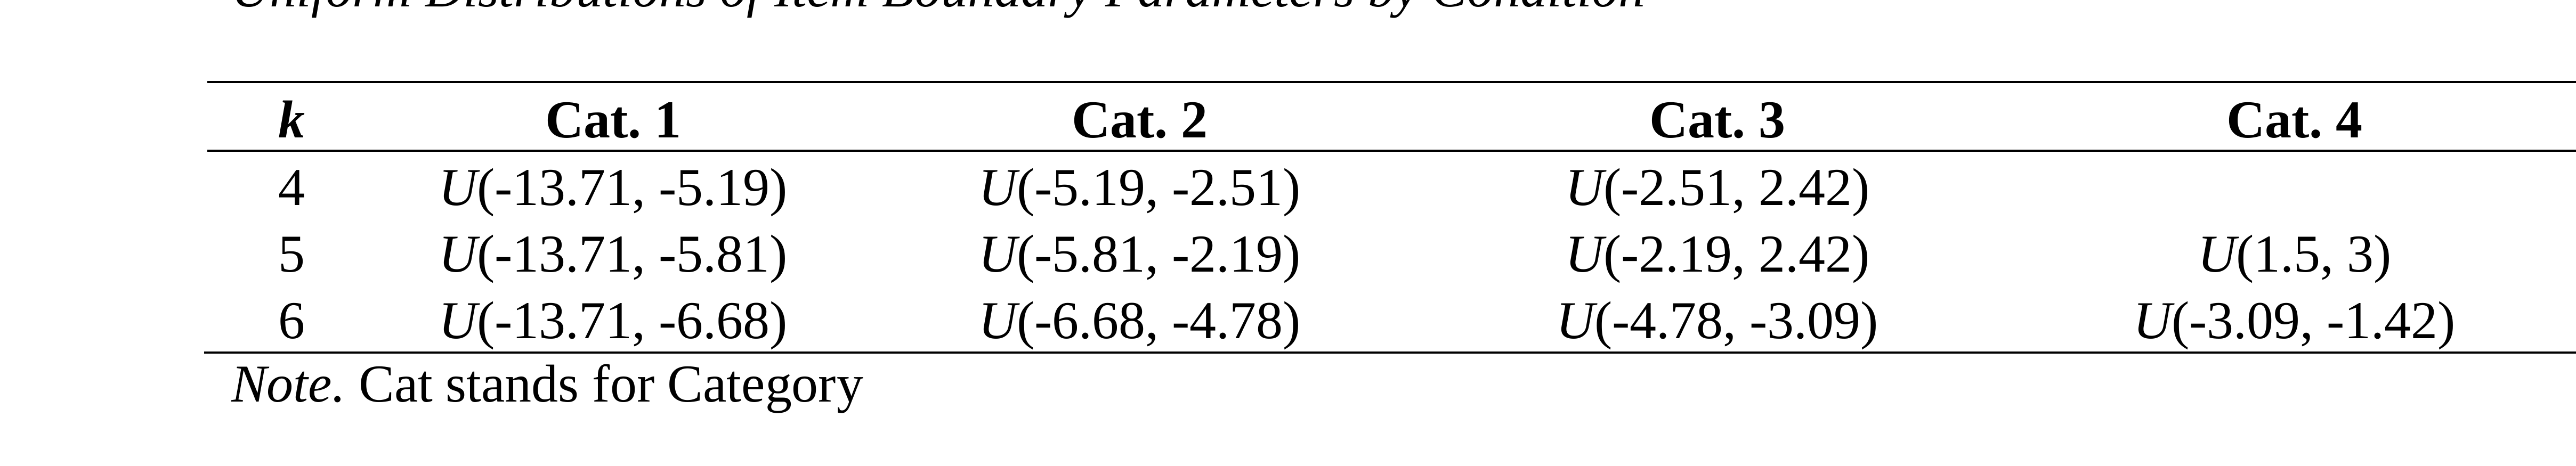
\includegraphics[width=0.92\textwidth]{figures/table_a2.png}
\caption{Table~A2. The \(k=7\) row is absent. For \(k=5\), category~3
and category~4 overlap.}
\label{fig:a2}
\end{figure}

\subsection{One draw of the boundaries, then a sort}

Table~A2 gives distributions.
The realized boundaries are not printed, and no seed is printed.
The run draws each boundary once from its interval under seed
\(20230511\), then sorts the boundaries within each item so they
increase.
For four and six options the intervals share only endpoints, so the
sort does not move an interior draw.
For five options, category~3 is \(U(-2.19, 2.42)\) and category~4 is
\(U(1.5, 3)\), so independent draws can arrive out of order.
The item indices in each of the \(32\) static tests are
\src{simulation/out/item_samples.csv}.

\subsection{Careless replacement of every item}

The dissertation says a uniform random option replaces the raw response
on the selected items, and that each option is equally likely.
It does not say how many items are selected.
The reported run replaces every item.
Replacing a fraction \(0.5\), \(0.2\), or \(0.1\) of the items leaves
the careless Guttman sensitivity at \(0.500\), \(0.485\), and \(0.444\),
against the printed \(0.29\).
The gap does not close under those fractions.
The files are the \texttt{c0.5}, \texttt{c0.2}, and \texttt{c0.1}
tables in \srcdir{simulation/out}.

\subsection{The sample standard deviation in the shift}

Equations~24 and~25 add or subtract \(s_{\delta_i}\), the standard
deviation of item \(i\)'s boundaries.
The run uses the sample standard deviation, with divisor \(n-1\).
Figure~\ref{fig:eq24} is the printed shift.

\begin{figure}[ht]
\centering
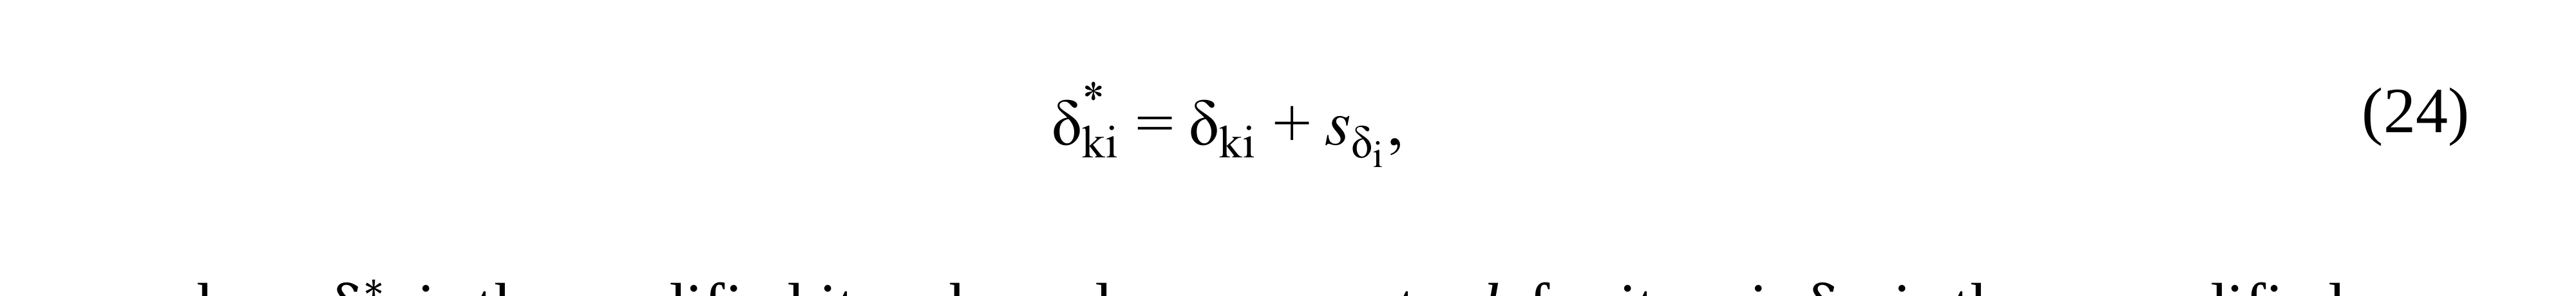
\includegraphics[width=0.85\textwidth]{figures/eq24.png}
\caption{Equation~24, the acquiescence shift.}
\label{fig:eq24}
\end{figure}

\subsection{Scaling constant D = 1}

The paragraph under Equation~23 calls \(D=1.702\) optional and
\(D=1\) the other choice.
The run uses \(D=1\), which is the logistic metric of
\texttt{mirt}'s graded generator.

\subsection{One latent sample, then a trim to 900}

The dissertation draws \(1{,}000\) latent vectors, drops zero-variance
response rows, and then drops rows at random until \(900\) remain.
The run draws one shared sample of \(1{,}000\) from the Table~A1 normal
distribution and trims each of the \(32\) response matrices separately.
The means and covariances are Figure~\ref{fig:a1}.
The socially desirable means are the four printed values in
Figure~\ref{fig:sdr}, with the same covariance.

\begin{figure}[ht]
\centering
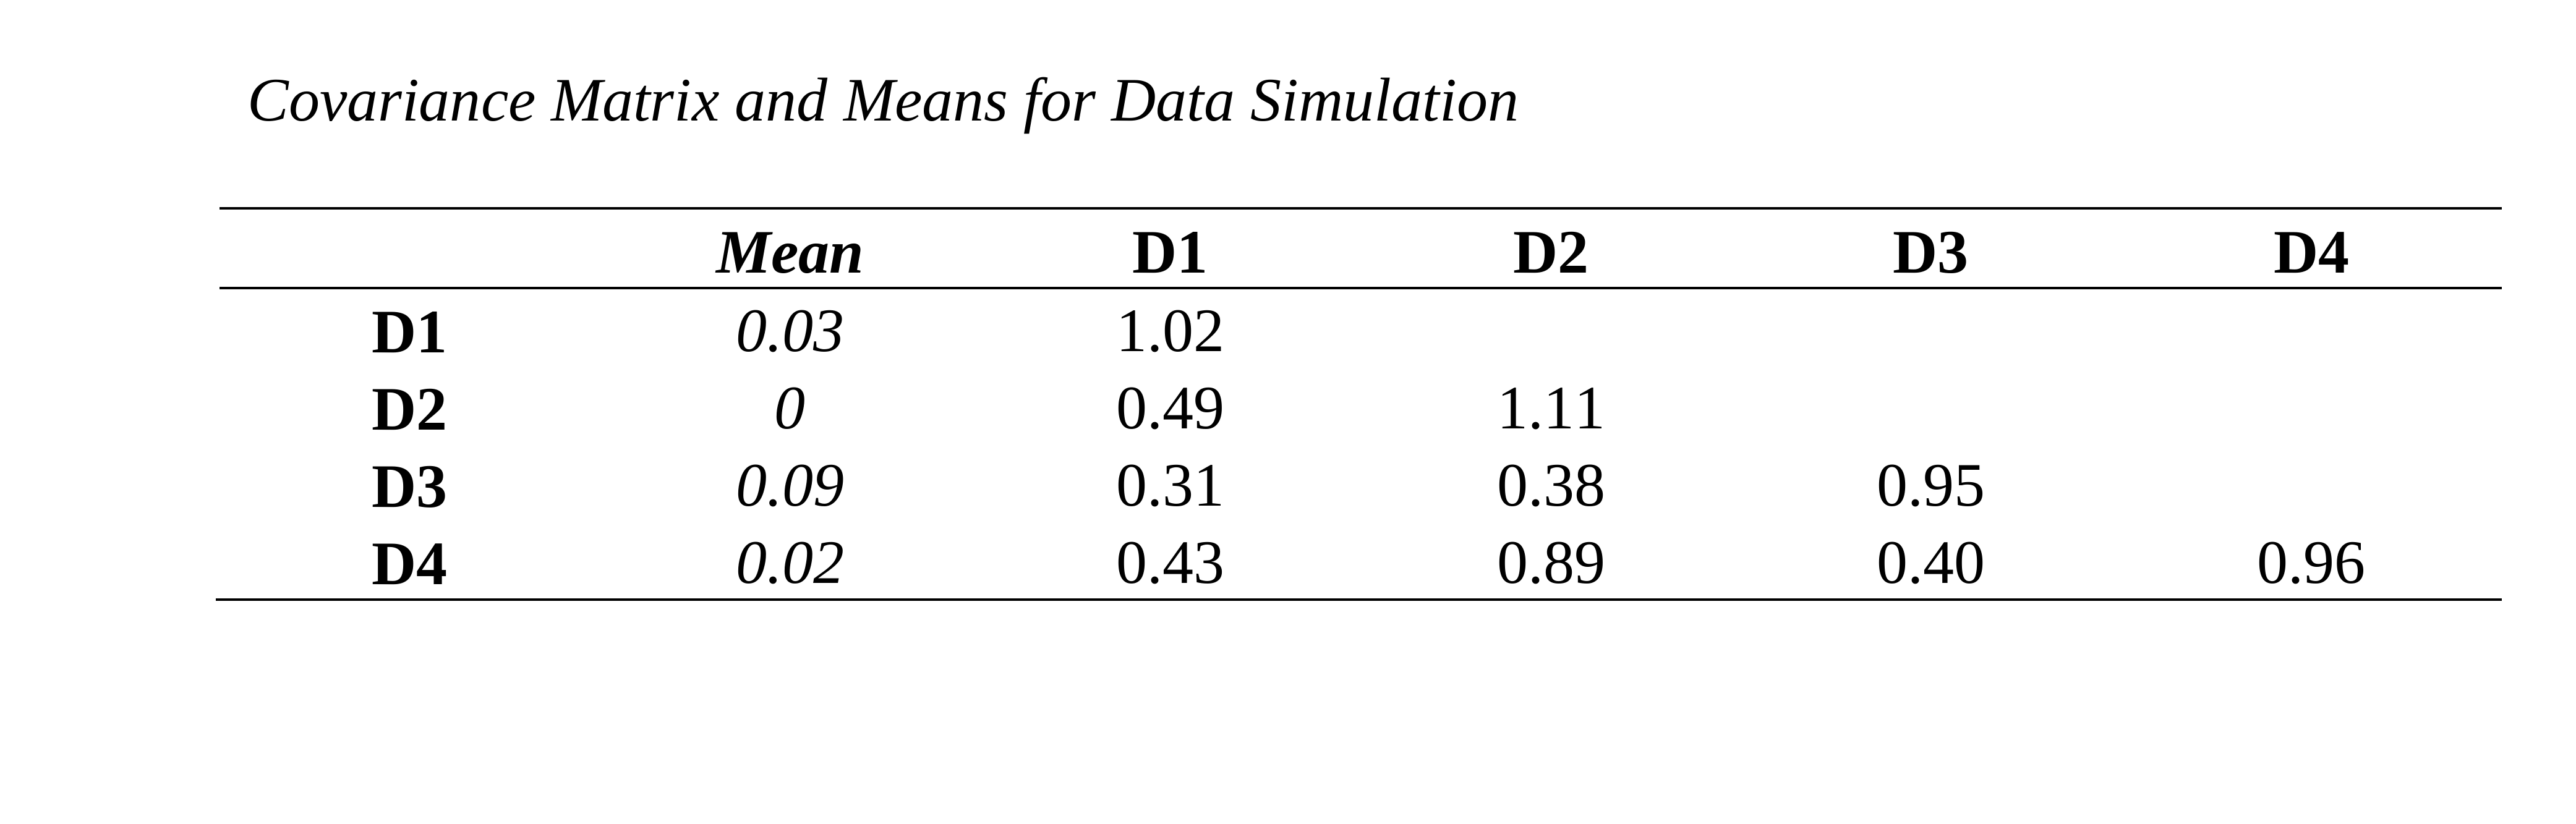
\includegraphics[width=0.85\textwidth]{figures/table_a1.png}
\caption{Table~A1. The matrix is positive definite, with eigenvalues
\(2.52\), \(0.71\), \(0.67\), and \(0.14\).}
\label{fig:a1}
\end{figure}

\begin{figure}[ht]
\centering
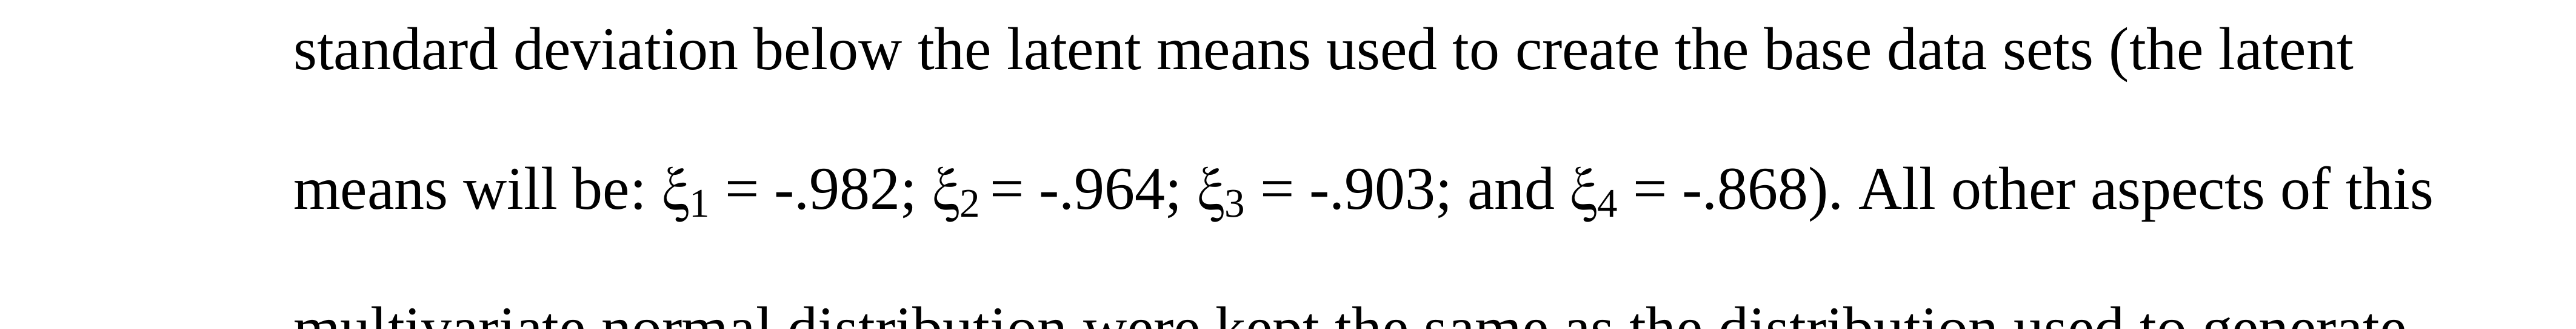
\includegraphics[width=0.92\textwidth]{figures/sdr_means.png}
\caption{The socially desirable means on page~66.}
\label{fig:sdr}
\end{figure}

\subsection{A sample quantile in place of the bootstrap median}

The dissertation takes the median of \(1{,}000\) bootstrap 5th
percentiles.
The run uses R's type-7 sample quantile at \(0.05\) or \(0.95\).
On one continuous sample of size \(1{,}000\), that median and the sample
5th percentile differ by \(3\times 10^{-4}\).
On a sample with a point mass, they differ by \(6\times 10^{-4}\).
The file is \src{simulation/out/bootstrap_cutoff.csv}, from
\src{simulation/bootstrap_cutoff.R}.
The comparison bands are an order of magnitude larger than those gaps
only for the careless ceiling, where the standard error is
\(5\times 10^{-5}\).
Elsewhere the quantile substitution is smaller than the band and does
not account for the misses.

\section{Ambiguities that were resolved}
\label{sec:resolved}

This section answers which readings of the page were settled by an
artifact.
Each subsection names the script, the output, and the command.
The commit that contains them is the commit that added this note.
Regenerate with the commands in \src{README.md}.

\subsection{Equation 23 is the sum that multiplies the threshold by each slope}

Figure~\ref{fig:eq23} prints
\[
P_{jk}(\theta)=\frac{1}{1+\exp\bigl[-D\sum_{h=1}^{H} a_{jh}(\theta_h-b_{jk})\bigr]}.
\]
The usual graded predictor, and \texttt{mirt}'s, is
\(a^\top\theta-b_{jk}\).
The printed sum equals \(a^\top\theta-b_{jk}\sum_h a_{jh}\).
The rerun passes \texttt{mirt} the intercept \(-b_{jk}\sum_h a_{jh}\).
Under the usual intercept \(-b_{jk}\), the trim to \(900\) non-constant
rows fails on the grid: a direct run stopped with fewer than \(900\)
such rows in the cells it reached.
A single twelve-item slice under that usual intercept has \(703\)
non-constant rows out of \(1{,}000\).
The same slice under the printed sum has \(754\).
The full printed-sum grid does trim to \(900\) in every cell.
The script is \src{simulation/standard_collapse.R}.
The generator is \srcat{simulation/monte_carlo.R}{108}.

\begin{figure}[ht]
\centering
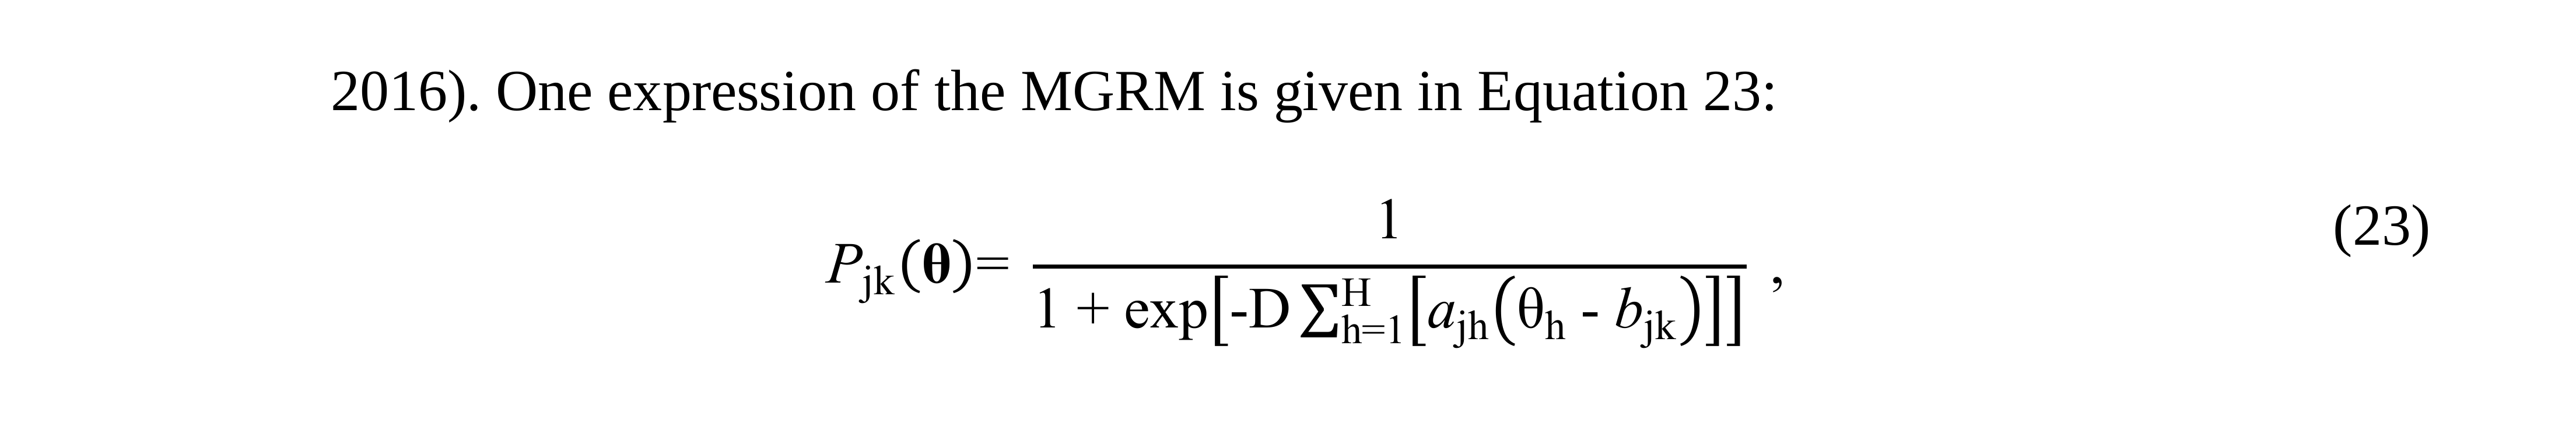
\includegraphics[width=0.92\textwidth]{figures/eq23.png}
\caption{Equation~23 as printed.}
\label{fig:eq23}
\end{figure}

\subsection{The aberrant tail is the high tail for U3 and for Guttman errors}

PerFit documents both statistics as increasing in misfit, from \(0\) to
\(1\).
\(H_i^T\) is low when a person is less scalable.
The method chapter states one 5th-percentile rule for all three.
Flagging the low tail of the normed Guttman errors, where many
respondents share a value at the quantile, flags about \(283\) people
rather than about \(50\), and the careless sensitivity on that tail is
\(0\).
Flagging the high tail flags about \(51\) people.
The high tail is the reading in Table~\ref{tab:guttman}.
The low tail is in the same output file, under the column prefix
\texttt{G\_lower}.

\subsection{Table A1 is the lower triangle including the variances}

The prose says the off-diagonal covariances run from \(0.31\) to
\(1.11\).
Figure~\ref{fig:a1} places \(1.11\) on the diagonal of the second
dimension, and places \(0.49\), \(0.31\), \(0.38\), \(0.43\), \(0.89\),
and \(0.40\) off the diagonal.
The simulation uses the figure.
The prose on the same page says the means run from \(-0.001\) to
\(0.092\).
The figure prints \(0\), \(0.02\), \(0.03\), and \(0.09\).
The simulation uses the figure.

\subsection{The package scores match the fast formulas}

\texttt{mokken::coefH} with standard errors on a \(36\times 1{,}000\)
matrix exhausted memory in this environment.
The \texttt{se = FALSE} branch is a covariance and a covariance of the
column-sorted matrix, and it finishes in a fraction of a second.
The validation command is \texttt{Rscript validate\_personfit.R out}.
The output is \src{simulation/out/validate_personfit.csv}.

\section{What remains unresolved}
\label{sec:open}

This section answers which gaps are still open, and which variations
were already run.

The eighteen grand sensitivities remain outside the two-standard-error
band after Holm.
The normed Guttman column has the same shape as the page: a floor at
midpoint responding, a high rate at extreme responding, and a ceiling
at careless responding.
The levels differ.
\(\varepsilon\in\{0.5, 1, 2\}\) moves the extreme rate through
\(0.284\), \(0.186\), and \(0.074\), against \(0.27\).
The value \(0.5\) is the closest of those three and is still \(0.014\)
above the page, with a standard error of \(0.00088\).
Careless fractions \(1\), \(0.5\), \(0.2\), and \(0.1\) leave that
sensitivity at \(0.500\), \(0.500\), \(0.485\), and \(0.444\), against
\(0.29\).
The fraction does not close the gap under this boundary draw.

\(U3\) remains a separate miss.
The statistic matches PerFit~1.4.7 before rounding.
On these replicates it does not track the printed \(U3\) column, which
tracks the printed Guttman column.
A different PerFit release from 2023, or a different boundary draw,
could still produce that tracking.
This run does not.

The realized boundaries, the item sample, and the seed are unprinted.
A different draw from Table~A2 can move a grand mean by more than the
Monte Carlo standard error of \(1{,}000\) replications, because that
standard error describes the redraw of the \(100\) biased respondents
with the items held fixed.
Our band uses our within-cell dispersion as a stand-in for theirs.
It is the right band for two runs of one fixed item set.
It is a lower bound on the uncertainty that comes from redrawing the
items.
The misses are large beside that lower bound: several hundredths, on
bands of about a thousandth.
Redrawing the items remains a live explanation, and so does the
unprinted \(\varepsilon\).

The sentence that the socially desirable means lie one standard
deviation below Table~A1 does not recover \(-0.982\), \(-0.964\),
\(-0.903\), and \(-0.868\).
The run uses those four printed numbers.

\section{What the 2015 thesis supplies}
\label{sec:thesis}

This section answers whether Beck (2015) \cite{beck2015} prints the
moments and the item slopes the dissertation says it adapted.
It prints scale means, scale correlations, and standardized factor
loadings.
It does not print graded-response boundaries.
Beck, Albano, and Smith (2019) \cite{beck2019} compare these statistics
on polytomous survey data.
The dissertation attributes the boundary and discrimination ranges to
fits in \texttt{ltm} \cite{rizopoulos2006}, not to that article.
An earlier request for the UTSA file returned HTTP 403.
The copy used here is the same bitstream, retrieved after that failure.
Its sha256 is
\sha{0425870dc5f65ce8ca1d0c0d80b646e12d81a4c8bf2b2cc0c5dc80084c98c707}.
The appendix numbers in the comparison are a transcription of the thesis
appendix, checked against the PDF (sha256
\sha{0425870dc5f65ce8ca1d0c0d80b646e12d81a4c8bf2b2cc0c5dc80084c98c707}).
Figure~\ref{fig:thesis} is Table~A4 of the thesis.

\begin{figure}[ht]
\centering
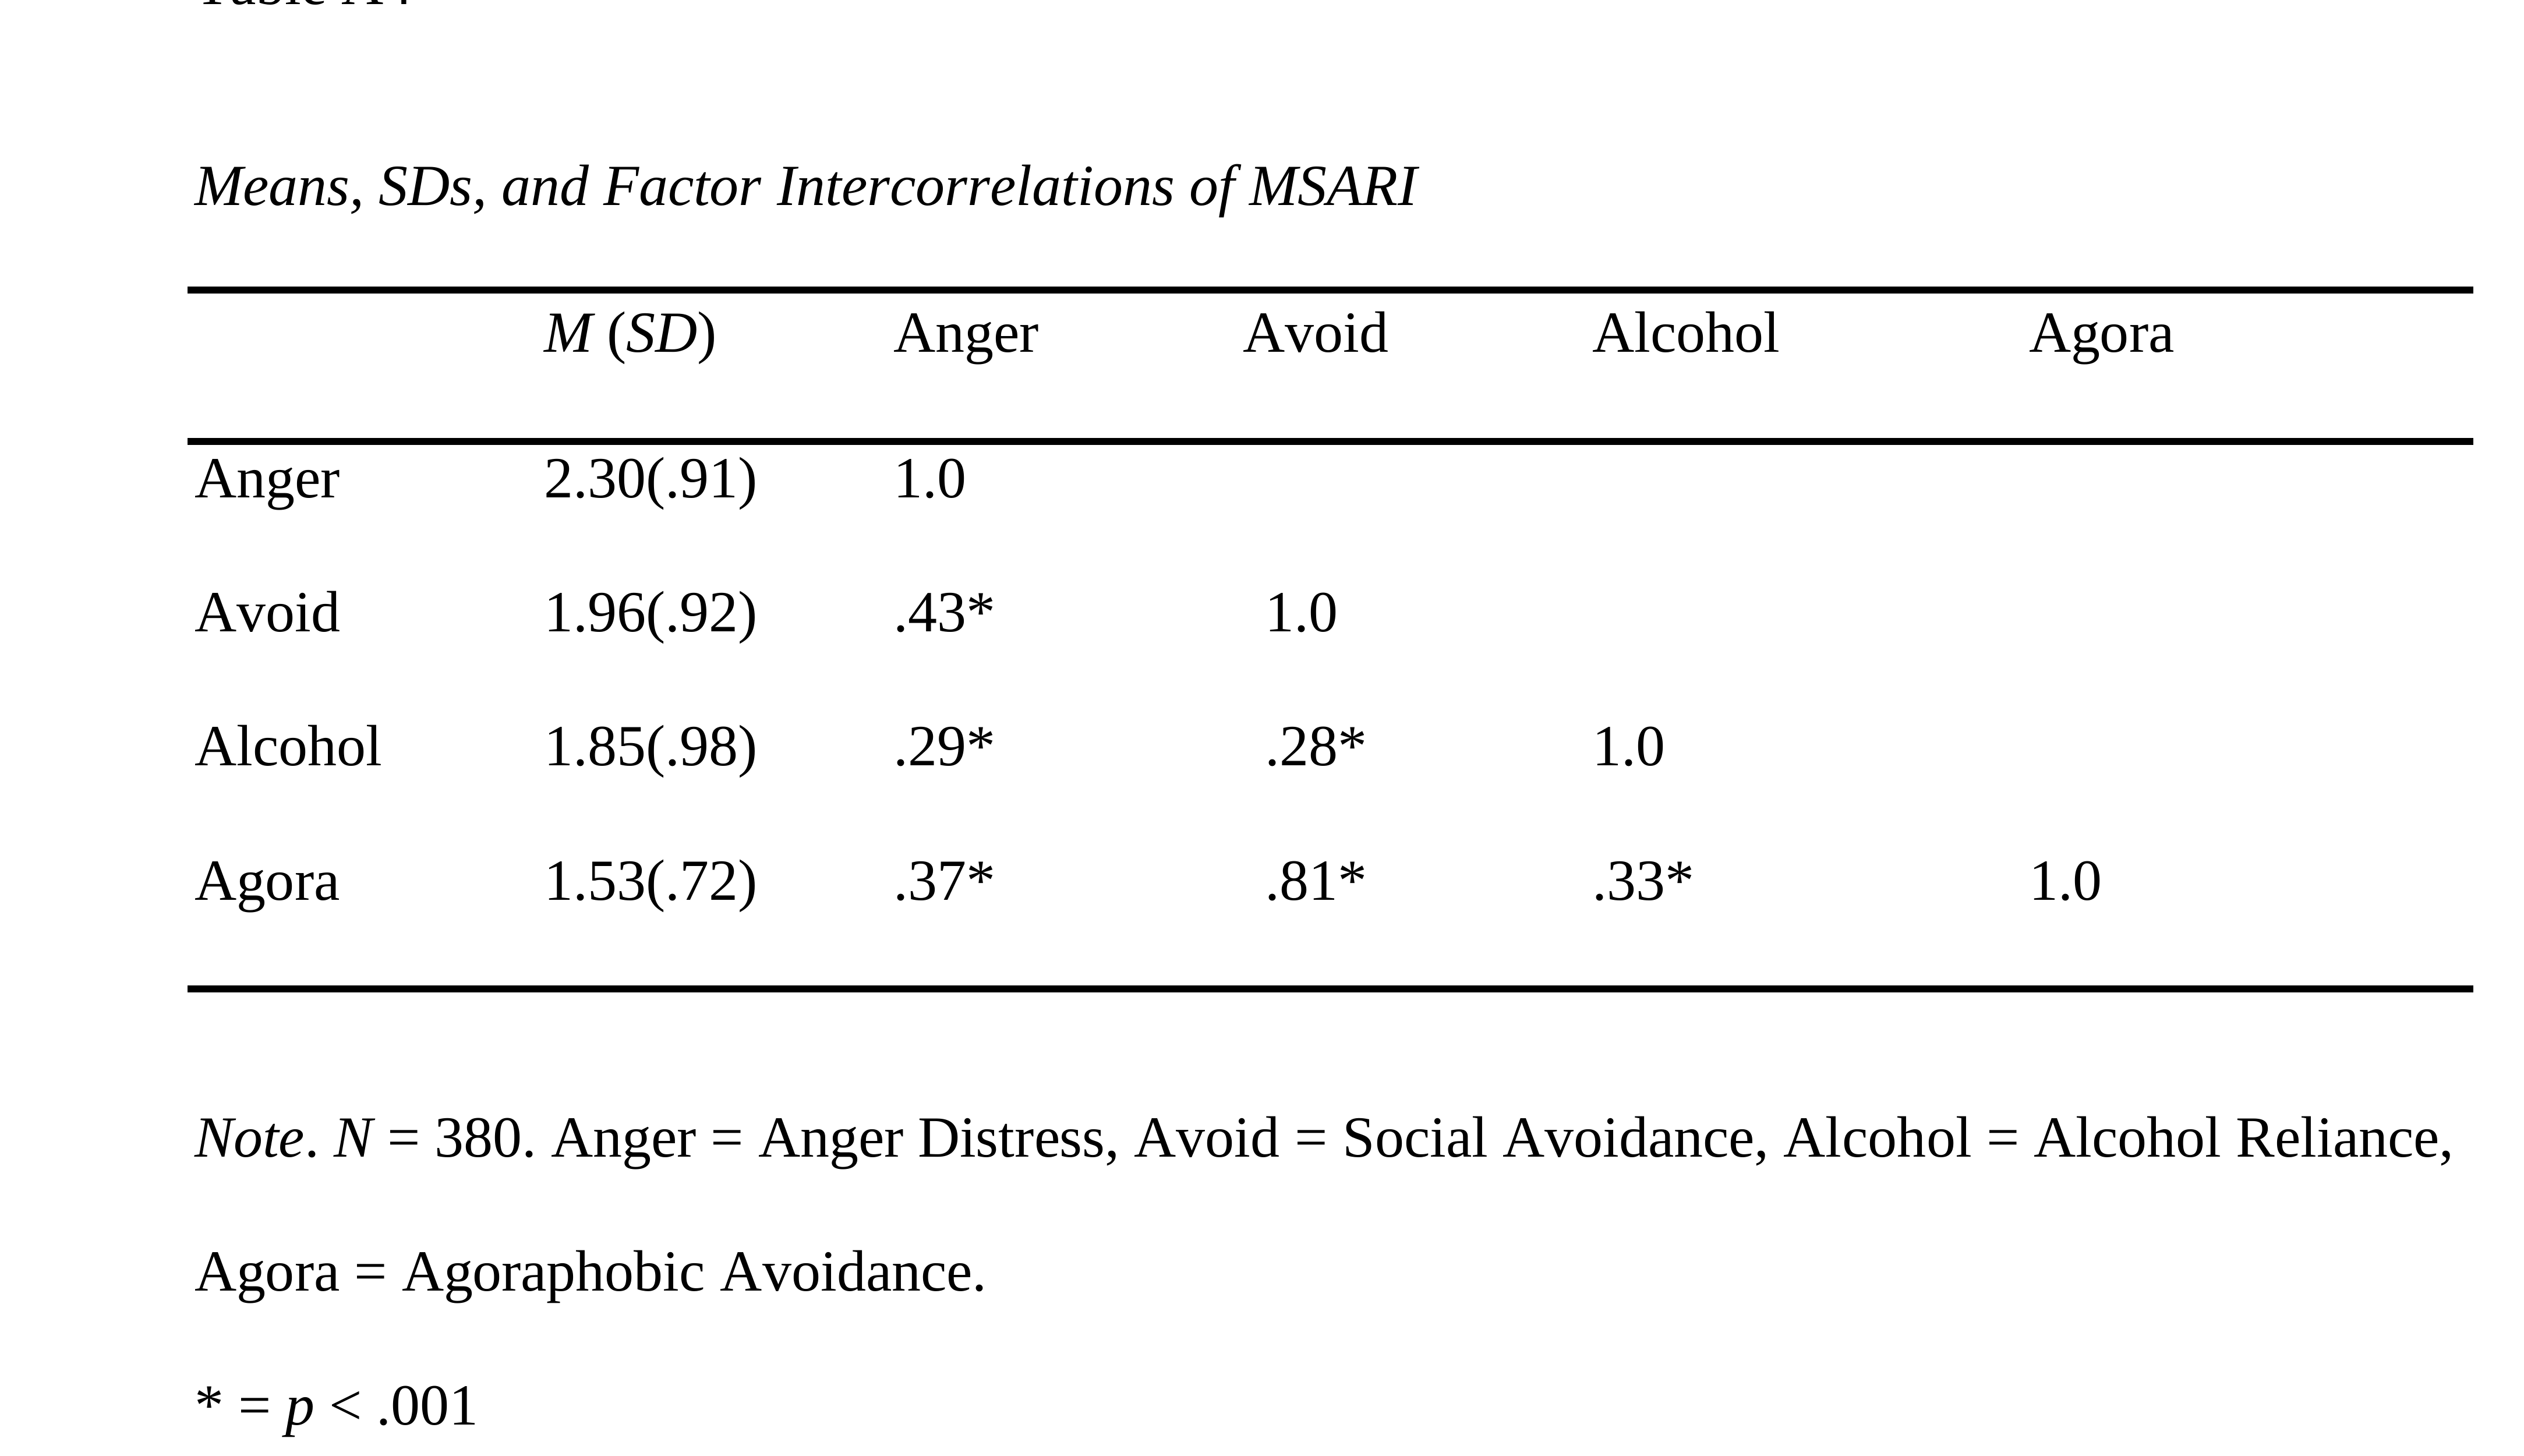
\includegraphics[width=0.92\textwidth]{figures/thesis_table_a4.png}
\caption{Beck (2015), Table~A4. Scale means, standard deviations, and
factor correlations for the MSARI-28. \(N=380\).}
\label{fig:thesis}
\end{figure}

The dissertation's Table~A1 is not this table.
The thesis correlations, in the order Anger, Avoid, Alcohol, Agora, are
\(0.43\), \(0.29\), \(0.37\), \(0.28\), \(0.81\), and \(0.33\).
The correlations implied by Table~A1, in the order printed there, are
\(0.46\), \(0.32\), \(0.43\), \(0.37\), \(0.86\), and \(0.42\).
The largest absolute difference is \(0.09\).
The scale-score covariance, using the printed standard deviations
\(0.91\), \(0.92\), \(0.98\), and \(0.72\), differs from Table~A1 by as
much as \(0.44\).
The scale means are \(2.30\), \(1.96\), \(1.85\), and \(1.53\).
Table~A1's means are near zero.
Substituting the scale means into the graded generator leaves every
cell with fewer than \(900\) non-constant base rows, so that reading
cannot be trimmed the way the dissertation describes.

Substituting the thesis correlations, with unit variances and means
zero, and with socially desirable means at \(-1\), does run.
At \(20\) replications and \(\varepsilon=0.5\), the normed-Guttman grand
sensitivities are \(0.063\), \(0.045\), \(0.004\), \(0.291\), \(0.032\),
and \(0.499\), against \(0.062\), \(0.047\), \(0.003\), \(0.284\),
\(0.031\), and \(0.500\) on Table~A1.
No grand sensitivity moves by as much as \(0.01\).
The file is \src{simulation/out/mc_ink_thesis_corr_eps0.5_c1_r20.csv}.

A slope \(a=\lambda/\sqrt{\psi}\) from a standardized loading \(\lambda\)
and residual \(\psi\), and the logistic form \(1.702\) times that slope,
were applied to the seven CFA loadings on each factor.
The logistic slopes run from \(1.28\) to \(3.76\).
The dissertation's stated uniforms run from \(1.80\) to \(6.65\), and
Table~A3 realizes slopes up to \(6.52\).
No assignment of the four factors puts the converted ranges on those
uniforms.
The conversion is \src{simulation/thesis_map.py} and
\src{simulation/out/thesis_lambda_to_a.csv}.
Those \(28\) logistic slopes, with Table~A1 and \(\varepsilon=0.5\)
held fixed, were run for eight replications.
One cell, seven options and one dimension at length \(12\), kept \(885\)
non-constant rows and was dropped.
On the other \(31\) cells the normed-Guttman grand sensitivities are
\(0.031\) for acquiescence, \(0.122\) for disacquiescence, \(0.001\) for
midpoint responding, \(0.292\) for extreme responding, \(0.017\) for
social desirability, and \(0.485\) for careless responding.
Disacquiescence moves from \(0.047\) on Table~A3 to \(0.122\), against
the printed \(0.13\).
The combined standard error is \(0.0017\), so the cell remains outside
the band.
Acquiescence moves from \(0.062\) to \(0.031\), away from the printed
\(0.05\).
Careless responding stays near the \(0.50\) ceiling.
The file is
\src{simulation/out/mc_ink_tablea1_thesis_cfa_eps0.5_c1_r8.csv}.

\section{Why the sensitivities miss}
\label{sec:why}

This section answers which missing input can account for the
sensitivity gaps, and which inputs were checked and set aside.
The ranking uses the size of the movement each input produced.

\begin{center}
\small
\renewcommand{\arraystretch}{1.3}
\begin{tabular}{@{}p{0.22\textwidth}p{0.36\textwidth}p{0.34\textwidth}@{}}
\toprule
Cause & Evidence for it & Evidence against it \\
\midrule
Extreme-response constant &
Extreme Guttman sensitivity moves from \(0.074\) at \(\varepsilon=2\) to \(0.284\) at \(\varepsilon=0.5\), toward the printed \(0.27\). &
The closest of those three values is still \(0.014\) outside a band of width \(0.0018\). Acquiescence, disacquiescence, social desirability, and careless responding do not use \(\varepsilon\), and they miss. \\
Item slopes and boundaries &
Table~A3 slopes reach \(6.52\). Converting the thesis loadings gives slopes from \(1.28\) to \(3.76\). Using those slopes moves disacquiescence from \(0.047\) to \(0.122\), against \(0.13\). &
The converted ranges are not the stated uniforms. The same run moves acquiescence from \(0.062\) to \(0.031\), away from \(0.05\), and careless responding stays at \(0.485\). The thesis has no graded thresholds. \\
Careless-item fraction &
The page does not say how many items are replaced. &
Fractions \(1\), \(0.5\), \(0.2\), and \(0.1\) leave the rate between \(0.44\) and \(0.50\), against \(0.29\). \\
Unprinted boundary draw &
The band is for one fixed item set. A new draw from Table~A2 is a different experiment. &
The gaps are several hundredths. That is possible for one unlucky draw, and it is large beside the redraw of the \(100\) biased respondents. \\
Latent covariance &
The dissertation says the moments were adapted from Beck (2015). &
The thesis correlations move the six Guttman rates by less than \(0.01\). \\
\(U3\) implementation &
The printed \(U3\) column tracks the Guttman column. Our \(U3\) does not. &
Our \(U3\) matches PerFit~1.4.7 and PerFit~1.4.6 before those packages round to four decimals. The Guttman misses do not depend on \(U3\). \\
Generator and the trim to \(900\) &
The usual \texttt{mirt} intercept, and the thesis scale means, both fail the trim. &
The printed-sum generator with Table~A1 completes the trim and still misses. A hand-written sampler matches \texttt{mirt}'s category probabilities to \(2\times 10^{-16}\) and its grand sensitivities to within \(0.0041\). \\
Bootstrap median versus the sample quantile &
The dissertation uses the bootstrap median. &
On two samples of size \(1{,}000\) the two cutoffs differ by \(3\times 10^{-4}\) and \(6\times 10^{-4}\). \\
Flagging direction &
The low tail of the normed Guttman errors flags about \(283\) people and gives careless sensitivity \(0\). The high tail flags about \(51\) and puts midpoint responding on the floor, which is the shape on the page. &
The high tail is the comparison in Table~\ref{tab:guttman}, and the level gaps remain on that tail. \\
\bottomrule
\end{tabular}
\end{center}

The first row is the strongest lever that was actually in our hands,
and it does not close the column.
The slope and boundary row is the live remainder: the thesis does not
contain the thresholds the dissertation says were fit with \texttt{ltm}~\cite{rizopoulos2006}.

\section{A second generator, and the May 2023 packages}
\label{sec:two}

This section answers whether the sensitivity misses are the choice of
\texttt{mirt::simdata} or the 2025 release of PerFit.
They are not.
No grand sensitivity enters the two-standard-error band under the
second generator.

The hand-written sampler is
\srcat{simulation/monte_carlo.R}{172}.
It draws one uniform per person and item from the linear predictor in
Equation~23.
Its category probabilities match \texttt{mirt} with a maximum absolute
difference of \(2\times 10^{-16}\), in
\src{simulation/out/generator_probs.csv}.
The same \(40\) replications, the same \(192\) conditions, and the same
four rates were then drawn with that sampler.
Against the printed tables, none of the eighteen aberrant-direction
grand sensitivities, and none of the matching specificity, positive
predictive value, or negative predictive value rows, fall inside the
band, before or after Holm.
The file is \src{simulation/out/comparison_hand_all.csv}.
The two generators' grand sensitivities differ by at most \(0.0041\).
Eight of those eighteen pairs sit outside two standard errors of each
other.
Three of the eight have a \(z\) between \(2\) and \(3\), and Holm brings
those three inside.
Five remain outside.
The largest absolute gap is extreme responding on the normed Guttman
errors, \(0.284\) on the \texttt{mirt} stream and \(0.280\) on the
hand-written stream, both against the printed \(0.27\).
Careless responding on that statistic differs by \(0.0003\) and is one
of the five, because both rates sit on \(0.50\) and the standard error
is about \(6\times 10^{-5}\).
On the other three rates the largest absolute gap is \(0.0089\), for
\(H_i^T\) positive predictive value under acquiescence.
The comparison is \src{simulation/out/generator_compare.csv}.

PerFit~1.4.6, dated 15~October~2021, was the release current through
May~2023.
PerFit~1.4.7 is the 2025 release used in the first grid.
\texttt{Gnormed.poly} and \texttt{U3poly} are the same in the two
releases.
mokken~3.0.6, dated 8~March~2021, was current until mokken~3.1.0 on
26~June~2023.
Its \texttt{coefH} branch with standard errors turned off is the same
rearrangement as mokken~3.1.2.
\texttt{mirt}~1.39 was packaged on 29~May~2023 (Pacific).
Its \texttt{simdata} body differs from \texttt{mirt}~1.36 by one
example, and the two \texttt{src} trees match.
Eight complete matrices, with four, five, six, and seven options and
with \(12\) and \(36\) items, scored by PerFit~1.4.6 and by mokken~3.0.6,
match the fast functions that match the later packages.
Every maximum absolute difference in
\src{simulation/out/version_check.csv} is \(0\).
The \(40\)-replication grid is already scored by those functions.
Installing the May~2023 releases and rescoring matrices of this
design's sizes therefore does not move a rate.
No grand sensitivity enters the band under those releases.
A second random grid under the old package names would redraw the
respondents.
It would not change the scoring rule that produced the misses.

\section{Which checks were run}
\label{sec:audit}

This section answers which of the checks that have closed gaps in
earlier replications were applied here.

\begin{center}
\small
\renewcommand{\arraystretch}{1.3}
\begin{tabular}{@{}p{0.28\textwidth}p{0.14\textwidth}p{0.48\textwidth}@{}}
\toprule
Check & Before this note's follow-up & Result \\
\midrule
Reread the displayed equations and tables &
Yes &
Equation~23, Table~A1, and Table~A2 match the page images. The \(k=7\) row is absent. \\
Swap one assumption at a time &
Epsilon and the careless fraction &
Thesis correlations and the loading-to-slope map were added. Correlations move rates by less than \(0.01\). The slopes move disacquiescence close to the printed value and move acquiescence away from it. \\
Back-solve the unprinted constant from the margins &
Yes, three values of \(\varepsilon\) &
\(0.5\) is the closest for extreme responding and remains outside the band. \\
Match the person-fit code to the packages &
Yes &
\(H_i^T\) matches \texttt{mokken}. \(U3\) and the normed Guttman errors match PerFit~1.4.7 before rounding. \\
Hand-written generator against \texttt{mirt} &
Probabilities only &
Full \(40\)-replication grid now run. Probabilities match to \(2\times 10^{-16}\). No grand sensitivity enters the printed band. The largest generator gap on a grand sensitivity is \(0.0041\). \\
Package versions from May~2023 &
No &
PerFit~1.4.6 and mokken~3.0.6 are the releases current then. \texttt{mirt}~1.39 (29~May~2023, Pacific) has the same \texttt{simdata} body and the same \texttt{src} as 1.36, apart from one example. Same-matrix score differences are \(0\). The grid is already scored by those functions, so no grand sensitivity enters the band. \\
More replications &
\(40\) &
The combined standard errors on the grand rates are about \(10^{-3}\) or smaller. A gap of \(0.01\) stays outside two standard errors at any larger replication count. \\
\bottomrule
\end{tabular}
\end{center}

The bootstrap-median cutoff was checked on two artificial samples, not
on every replication of the grid.
The differences were \(3\times 10^{-4}\) and \(6\times 10^{-4}\).

\section{Conclusion}
\label{sec:conclusion}

This section answers whether the dissertation's headline detection
rates were recovered.
They were not.
None of the eighteen grand sensitivities fall inside a
two-standard-error band, before or after Holm.
Careless responding comes out between \(0.44\) and \(0.50\), against
the printed \(0.29\).
The nearest misses, at \(\varepsilon=0.5\), are the normed Guttman
errors for midpoint responding, \(0.0035\) against \(0.00\), and for
extreme responding, \(0.284\) against \(0.27\).
The likely causes are unpublished inputs: the \texttt{ltm} thresholds
and the seven-option row, the boundary draw and its seed, the
extreme-response constant, and the careless fraction.
The generator, the package versions current in May~2023, Monte Carlo
noise, and the person-fit implementations do not account for the
misses.
The ANOVA effect sizes do replicate: all \(504\) partial omega squared
values agree with the printed \(F\) statistics at \(N=32{,}000\), to
within \(0.005\).
Specificity, negative predictive value, and positive predictive value
largely follow from flagging \(5\%\) of respondents, and in the printed
tables they sit close to that identity.

\section{Code and source availability}
\label{sec:availability}

This section answers where the inputs and the outputs live.
The dated ledger is in \src{INVESTIGATION.md}.

The dissertation is Beck (2023) \cite{beck2023},
\url{https://digitalcommons.unl.edu/cehsdiss/425}.
The PDF used here has sha256
\sha{86c3bb482efadc385cd52f7ea12dc33c50b9b70b4ce6111aedb075a12968f62b}.
It is the Wayback snapshot \texttt{20240907085051} of
\url{https://digitalcommons.unl.edu/cgi/viewcontent.cgi?article=1436&context=cehsdiss}.
A direct request for that URL on 28~October~2026 returned a Cloudflare
challenge page.
The PDF is not in git.

The thesis is Beck (2015) \cite{beck2015},
\url{https://rrpress.utsa.edu/server/api/core/bitstreams/4fbd58d2-5896-4dea-ab69-300c5c676a07/content},
ProQuest No.~1588285.
An earlier fetch of that file returned HTTP 403.
The copy obtained after that failure has sha256
\sha{0425870dc5f65ce8ca1d0c0d80b646e12d81a4c8bf2b2cc0c5dc80084c98c707}.
It is not in git.
The loadings used in Section~\ref{sec:thesis} are a transcription of the
thesis appendix, checked against the PDF (sha256
\sha{0425870dc5f65ce8ca1d0c0d80b646e12d81a4c8bf2b2cc0c5dc80084c98c707}).

No sentence in the dissertation names a script archive.
The public GitHub account \texttt{MFBeck} has two repositories,
\texttt{Hello\_Jenkins} and \texttt{jenkins\_test}, cloned on
28~October~2026; both are Jenkins demonstrations.
An OSF search, a Zenodo search, and a GitLab search on that date did
not return a simulation archive for this dissertation.
PerFit's source for the two polytomous statistics is the repository
\url{https://github.com/jorgetendeiro/PerFit}, version 1.4.7.

\section{Next steps}
\label{sec:next}

This section answers what would replace an assumption with a printed
input.
The 2015 thesis is in hand and does not print the graded thresholds.
A seed, the \texttt{ltm} \cite{rizopoulos2006} boundary matrix, or an R \texttt{sessionInfo}
record from the dissertation run would decide whether the sensitivity
gaps are that unpublished fit.
The check is the same Monte Carlo with those inputs in place of seed
\(20230511\) and of \(\varepsilon=0.5\).

\section{Artifacts}
\label{sec:artifacts}

This section lists each claim, the file that holds it, and the command
that regenerates it.
Commands run from \texttt{formalization/polytomous-person-fit/simulation}
unless the path says otherwise.
The PDF path below is the copy named in Section~\ref{sec:availability}.

\begin{center}
\small
\begin{tabular}{@{}p{0.28\textwidth}p{0.32\textwidth}p{0.32\textwidth}@{}}
\toprule
Claim & File & Command \\
\midrule
Discriminations, Tables~A6--A26, Tables~C1--C18 &
\src{simulation/out/discriminations.csv} and the published CSV files &
\texttt{python3 extract\_published.py PDF out} \\
Omega squared from the printed \(F\) &
\src{simulation/out/anova_check.csv} &
the same command \\
Identity residuals &
\src{simulation/out/identity_residuals.csv} &
the same command \\
Package agreement &
\src{simulation/out/validate_personfit.csv} &
\texttt{Rscript validate\_personfit.R out} \\
Forty replications, \(\varepsilon=0.5\) &
\src{simulation/out/mc_ink_eps0.5_c1_r40.csv} &
\texttt{Rscript monte\_carlo.R out 40 ink 0.5 4 1} \\
Forty replications, \(\varepsilon=1\) &
\src{simulation/out/mc_ink_eps1_c1_r40.csv} &
\texttt{Rscript monte\_carlo.R out 40 ink 1 4 1} \\
Comparison, \(\varepsilon=0.5\) &
\src{simulation/out/comparison_eps05.csv} &
\texttt{Rscript score\_gaps.R} on that file \\
Quantile against bootstrap median &
\src{simulation/out/bootstrap_cutoff.csv} &
\texttt{Rscript bootstrap\_cutoff.R out} \\
Loading-to-slope map &
\src{simulation/out/thesis_lambda_to_a.csv} &
\texttt{python3 thesis\_map.py} \\
Thesis correlations, 20 replications &
\src{simulation/out/mc_ink_thesis_corr_eps0.5_c1_r20.csv} &
\texttt{Rscript monte\_carlo.R out 20 ink 0.5 2 1 thesis\_corr} \\
CFA slopes, eight replications &
\src{simulation/out/mc_ink_tablea1_thesis_cfa_eps0.5_c1_r8.csv} &
\texttt{Rscript monte\_carlo.R out 8 ink 0.5 1 1 tablea1 thesis\_cfa} \\
Hand-written generator, 40 replications &
\src{simulation/out/mc_hand_ink_tablea1_tablea3_eps0.5_c1_r40.csv} &
\texttt{Rscript monte\_carlo.R out 40 ink 0.5 2 1 tablea1 tablea3 hand} \\
Hand generator against the printed tables &
\src{simulation/out/comparison_hand_all.csv} &
{\raggedright\texttt{Rscript score\_gaps.R out/}\allowbreak\texttt{mc\_hand\_ink\_tablea1\_}\allowbreak\texttt{tablea3\_eps0.5\_c1\_r40.csv}\ \texttt{out all}\ \allowbreak\texttt{comparison\_hand\_all.csv}\par} \\
Category probabilities, hand against \texttt{mirt} &
\src{simulation/out/generator_probs.csv} &
\texttt{Rscript check\_generator.R out} \\
Generator comparison &
\src{simulation/out/generator_compare.csv} &
{\raggedright\texttt{Rscript compare\_generators.R}\ \allowbreak\texttt{out/mc\_ink\_eps0.5\_c1\_r40.csv}\ \allowbreak\texttt{out/mc\_hand\_ink\_tablea1\_}\allowbreak\texttt{tablea3\_eps0.5\_c1\_r40.csv out}\par} \\
May 2023 package scores &
\src{simulation/out/version_check.csv} &
\texttt{Rscript version\_check.R out} \\
Crops &
\srcdir{paper/figures} &
\texttt{python3 paper/figures/crop\_pages.py PDF} \\
\bottomrule
\end{tabular}
\end{center}

\begin{thebibliography}{9}
\bibitem{beck2023}
M.~F. Beck.
\emph{The Examination of Nonparametric Person-Fit Statistics as
Appropriate Measures of Response Bias in Ordered Polytomous Items}.
Ph.D.\ dissertation, University of Nebraska--Lincoln, May 2023.
\url{https://digitalcommons.unl.edu/cehsdiss/425}.

\bibitem{beck2015}
M.~F. Beck.
\emph{The Multidimensional Social Anxiety Response Inventory (MSARI):
Development and Preliminary Examination of Psychometric Properties}.
Master's thesis, The University of Texas at San Antonio, 2015.
ProQuest No.~1588285.
\url{https://rrpress.utsa.edu/server/api/core/bitstreams/4fbd58d2-5896-4dea-ab69-300c5c676a07/content}.

\bibitem{beck2019}
M.~F. Beck, A.~D. Albano, and W.~M. Smith.
Person-fit as an index of inattentive responding: A comparison of
methods using polytomous survey data.
\emph{Applied Psychological Measurement}, 43:374--387, 2019.

\bibitem{rizopoulos2006}
D.~Rizopoulos.
ltm: An R package for latent variable modeling and item response
theory analyses.
\emph{Journal of Statistical Software}, 17(5):1--25, 2006.
\url{https://doi.org/10.18637/jss.v017.i05}.

\bibitem{rcore}
R Core Team.
\emph{R: A Language and Environment for Statistical Computing}.
R Foundation for Statistical Computing, Vienna, 2024.
Version 4.3.3.
\url{https://www.r-project.org/}.

\bibitem{chalmers2012}
P.~Chalmers.
mirt: A multidimensional item response theory package for the R
environment.
\emph{Journal of Statistical Software}, 48:1--29, 2012.
Version 1.36, 21~March~2022.
\url{https://cran.r-project.org/package=mirt}.

\bibitem{vanderark2012}
L.~A. van der Ark.
New developments in Mokken scale analysis in R.
\emph{Journal of Statistical Software}, 48:1--27, 2012.
Package \texttt{mokken}, versions 3.1.2 and 3.0.6.
\url{https://cran.r-project.org/package=mokken}.

\bibitem{tendeiro2016}
J.~N. Tendeiro, R.~R. Meijer, and A.~S.~M. Niessen.
PerFit: An R package for person-fit analysis in IRT.
\emph{Journal of Statistical Software}, 74:1--27, 2016.
Versions 1.4.7 and 1.4.6.
\url{https://cran.r-project.org/package=PerFit}.

\bibitem{venables2002}
W.~N. Venables and B.~D. Ripley.
\emph{Modern Applied Statistics with S}.
Springer, New York, 4th edition, 2002.
Package MASS, version 7.3-60.0.1.
\url{https://cran.r-project.org/package=MASS}.
\end{thebibliography}

\end{document}
